\label{sec:motivation}

\section{Function Prioritization Motivation}

\begin{table*}
  \caption{Delay-tolerant scenarios. The ID of the use case is taken from a public dataset~\cite{Eismann:zenodo:2021:dataset}. We studied each case and estimate a likely delay tolerance for that scenario.}
  \label{tab:examples}
  \centering
  \begin{tabular}{lrll}
    \toprule
    Trigger group & ID & Delay     & Description \\
                  &    & tolerance & \\
    \midrule
    timer & 6 & $<$10min & NetApp's cloud function to periodically find unutilized EBS volumes to delete. \\
    event & 28 & $<$60min & Google Analytics clone to track website visitors. \\ %Note from Cristina: Google Analytics updates statistics every 24-48 hours for standard accounts 
    queue & 59 & $<$60min & Messenger Chatbot for a media company; sends weekly news updates to user. \\
    storage & 30 & $<$10min & Serverless Galleria, for batch manipulation and publishing of images. \\
    orchestration & 12 & $<$24h & Subscription fulfillment for online and print subscriptions of The Guardian. \\
    others & 101 & $<$10min & Scientific task, batch, on demand, for sequence alignment of protein sequences. \\
  \bottomrule
\end{tabular}
\end{table*}

In this section, we show that---in opposition to what others have argued in the past~\cite{Wiesner:Middleware:2021:TemporalShifting}---(some) real serverless workloads \emph{are} delay tolerant (\S~\ref{sec:motivation:delay-tolerant}), we discuss the current status of differentiated serverless functions (\S~\ref{sec:motivation:currentStatus}) and provide a workload characterization based on dividing functions into high- and low-priority classes (\S~\ref{sec:motivation:workload}).
Our study of the delay tolerance of serverless functions is based on a recent dataset of serverless applications~\cite{Eismann:Software:2021:Why,Eismann:TSE:2021:CommunityConsensus}.
For the workload characterization, we analyze traces with real serverless workloads from Microsoft Azure~\cite{Shahrad:ATC:2020:ServerlessInTheWild} and present the results of one representative day (day 5 of the 2-week trace).
%we have released the code used for the analysis in this section.\footnote{GiHub link blinded for review.}

\subsection{Can Serverless Functions be Delayed?}
\label{sec:motivation:delay-tolerant}
In this subsection, we analyze if serverless functions can tolerate some level of delay in their execution. 
This delay could come from not executing the function immediately (e.g. through queueing), or via reduced priority in scheduling (e.g. giving less resources to lower-priority functions).
While these two mechanisms differ, the result of both is increasing the turnaround time of the functions; this increase is not appropriate for some functions---like those supporting interactive or real-time applications---but is tolerable for multiple other applications, as discussed in this subsection.

Serverless functions can be triggered through several mechanisms like http invocations, cloud-native events, queue messages and timers.
Functions triggered by http are time sensitive as these are synchronous requests that can timeout and are often used in interactive applications;
all other triggers invoke functions that can tolerate delays to varying degrees.
Thus, functions not triggered by http are (potentially) delayable; in the Azure trace, these constitute $59.06\%$ of the functions and $69.07\%$ of the invocations.

Furthermore, a recent survey of serverless use cases~\cite{Eismann:TSE:2021:CommunityConsensus} found that 66\% of applications in a large dataset have at least one delay-tolerant function.
To further illustrate our point, we analyzed the applications in the dataset and selected one delay-tolerant scenario for each of the triggers (except http, which is not delayable as already explained);
these scenarios are described in Table~\ref{tab:examples} and include examples such as removing unutilized EBS volumes, a web analytics (clickstream) application, a messenger chatbot, a batch image manipulation application for a serverless galleria, a subscription fulfillment application for The Guardian, and an application for sequence alignment of protein sequences.

A note on http-triggered functions: Some web applications need end users to invoke asynchronous behavior via http requests.
The Microsoft Azure Cloud Design Patterns documentation~\cite{Eastbury:2022:Azure:AsyncPattern} provides a solution to this problem with the ``Asynchronous Request-Reply'' pattern which disaggregates such behavior into three functions: two http-triggered ones (to enqueue request and to check status of job), and a queue-triggered backend function.
In this scenario, the http-triggered functions are not delay tolerant, but the queue-triggered function is.
%(though it may tolerate only a small delay depending on the specific use case).


\subsection{Current Status of Differentiated FaaS Invocations}
\label{sec:motivation:currentStatus}
A recent empirical study~\cite{Tariq:SOCC:2020:Sequoia} found that current cloud providers (AWS, Azure, GCP and IBM) treat http functions differently from those triggered by other means, frequently via undocumented behavior, including different concurrency limits and prioritization versus background functions.
In addition, while asynchronous functions are queued and thus the user understands that they may not execute immediately, providers don't typically enqueue synchronous functions but rather return with an error if peak exceeds concurrency limits or provider capacity.\footnote{An exception is GCP which handles synchronous calls in best effort fashion, performing queuing but not ensuring zero drops~\cite{Tariq:SOCC:2020:Sequoia}.}
%
Thus, the major public cloud providers are already implicitly defining two classes of functions: high priority (synchronous) and lower priority (asynchronous), with the latter being delay-tolerant.
%asynchronous functions in AWS can be queued up to 6 hours.\footnote{\url{https://docs.aws.amazon.com/lambda/latest/dg/invocation-async.html}}
%Asynchronous functions are either explicitly (for example, with the \texttt{async} keyword in OpenWhisk) or implicitly (by its trigger) defined in current platforms.
%The asynchronous functions are good candidates to be delayed if needed.

In OpenWhisk asynchronous functions are defined with the \texttt{async} keyword and follow a different execution path than synchronous ones.
However, the platform does not use any mechanism to delay or execute them at a lower priority.
A solution that treats \texttt{async} functions as delay-tolerant, scheduled with a lower priority than synchronous functions, can be added to OpenWhisk without API modifications.

\subsection{High- and Low-Priority Workloads}
\label{sec:motivation:workload}
%Re-write section: try to make more compact 1-2 paragraphs is better
Considering the two function classes described in the prior subsection---high and low priority---we analyze the Azure traces applying this division in the workload.
For the high priority class, we consider http-triggered functions.
For the low priority class, we consider all other functions.

%\paragraph{Prevalence in workload}
High-priority functions constitute a significant portion of the workload, though the low-priority functions are greater in number and account for more than 2/3 of the invocations.
Specifically, high-priority functions constitute $41\%$ of the functions and $31\%$ of the invocations, versus $59\%$ of the functions and $69\%$ of the invocations for the low-priority.
%Higher precision numbers:
%$40.94\%$,  $30.93\%$
%$59.06\%$, $69.07\%$ 

%\paragraph{Function duration}
Figure~\ref{fig:CDF:workload} (Left) shows the cumulative distribution function (CDF) of the average function durations.
%; the dataset does not contain the duration of each invocation, just per-function aggregate statistics.
The function durations are similar for both classes, with high-priority functions being slightly shorter (median 0.2 vs 0.8 minutes).
%\paragraph{Interarrivals}
Figure~\ref{fig:CDF:workload} (Right) shows the CDF of the per-function average inter-arrivals;
%The dataset contains arrivals aggregated at per-minute intervals, making it impossible to get low granularity statistics for interarrivals smaller than one minute; most (98.8\%) interarrivals fall in this category.
the IATs for both classes are similar.
%---at the granularity that we can do the analysis---

% \begin{figure}[t]
%     \centering
%     \includegraphics[width=0.8\columnwidth]{../Figures/CDF-functionDurationsByPriority.eps}
%     \caption{CDF of the function durations, with functions divided into two groups: high-priority and low-priority.}
%     \label{fig:CDF:durationByPriority}
% \end{figure}

\begin{figure}[t]
    \centering
    \begin{minipage}{0.49\linewidth}\vspace{0pt}%
        \includegraphics[width=\linewidth]{chrlu/qos/Figures/CDF-functionDurationsByPriority.eps}
    \end{minipage}
    \begin{minipage}{0.48\linewidth}\vspace{-5pt}%
        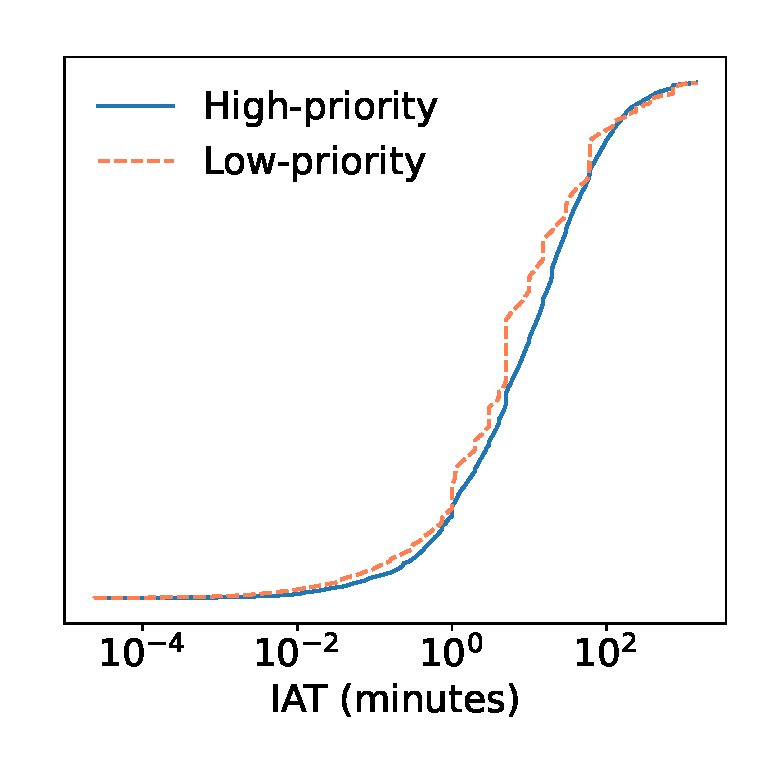
\includegraphics[width=0.95\linewidth]{chrlu/qos/Figures/CDF-averageInterarrivals.eps}
    \end{minipage}
    %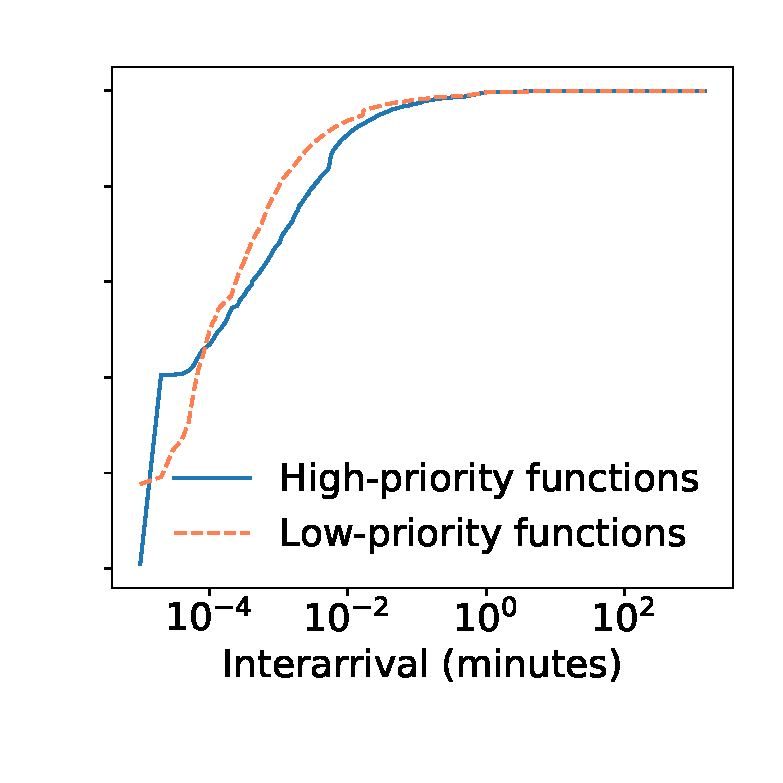
\includegraphics[width=0.49\columnwidth]{../Figures/CDF-interarrivals.eps}
    \caption{Left: CDF of the function durations. Right: CDF of the average function inter-arrivals. Functions are divided into two classes: high and low priority.}
    \label{fig:CDF:workload}
\end{figure}


% \begin{figure}[t]
%     \centering
%     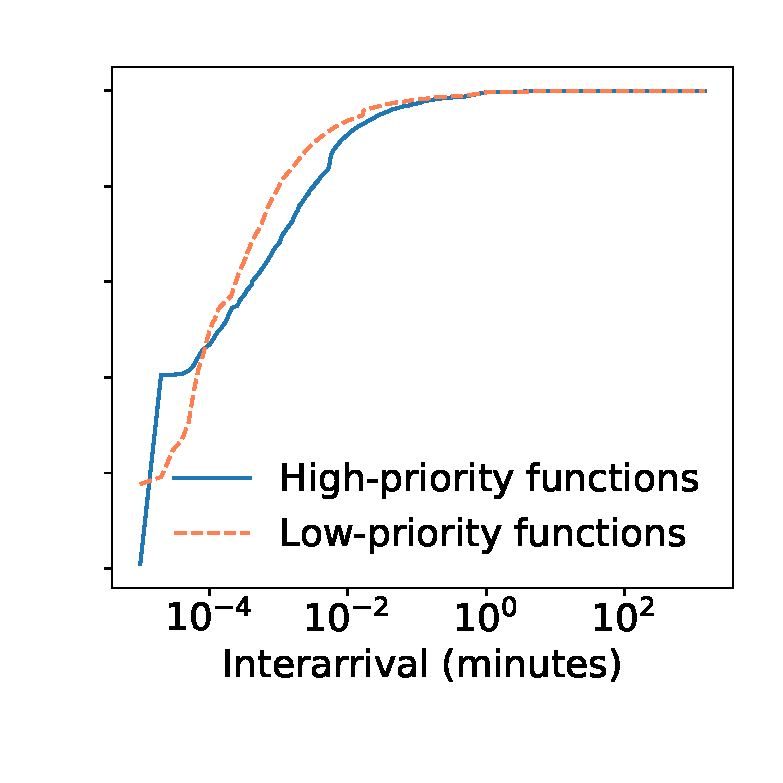
\includegraphics[width=0.8\columnwidth]{../Figures/CDF-interarrivals.eps}
%     \caption{CDF of the per-function interarrivals, with functions divided into two groups: high-priority and low-priority.}
%     \label{fig:CDF:interarrivalsByPriority}
% \end{figure}

\begin{comment}
\paragraph{Burstiness}
Figure~\ref{fig:bursty:highVsLowNormalized} shows the per-minute invocations, with functions divided into high and low priority groups and with invocations normalized to their peaks.
Both groups have similar burstiness: high-priority ($IDC=0.0083, \sigma=0.0794$) and low-priority ($IDC=0.0079, \sigma=0.0764$).
Even though the burstiness is similar, the peaks may or may not align during the 24-hour period.

\begin{figure}[t]
    \centering
    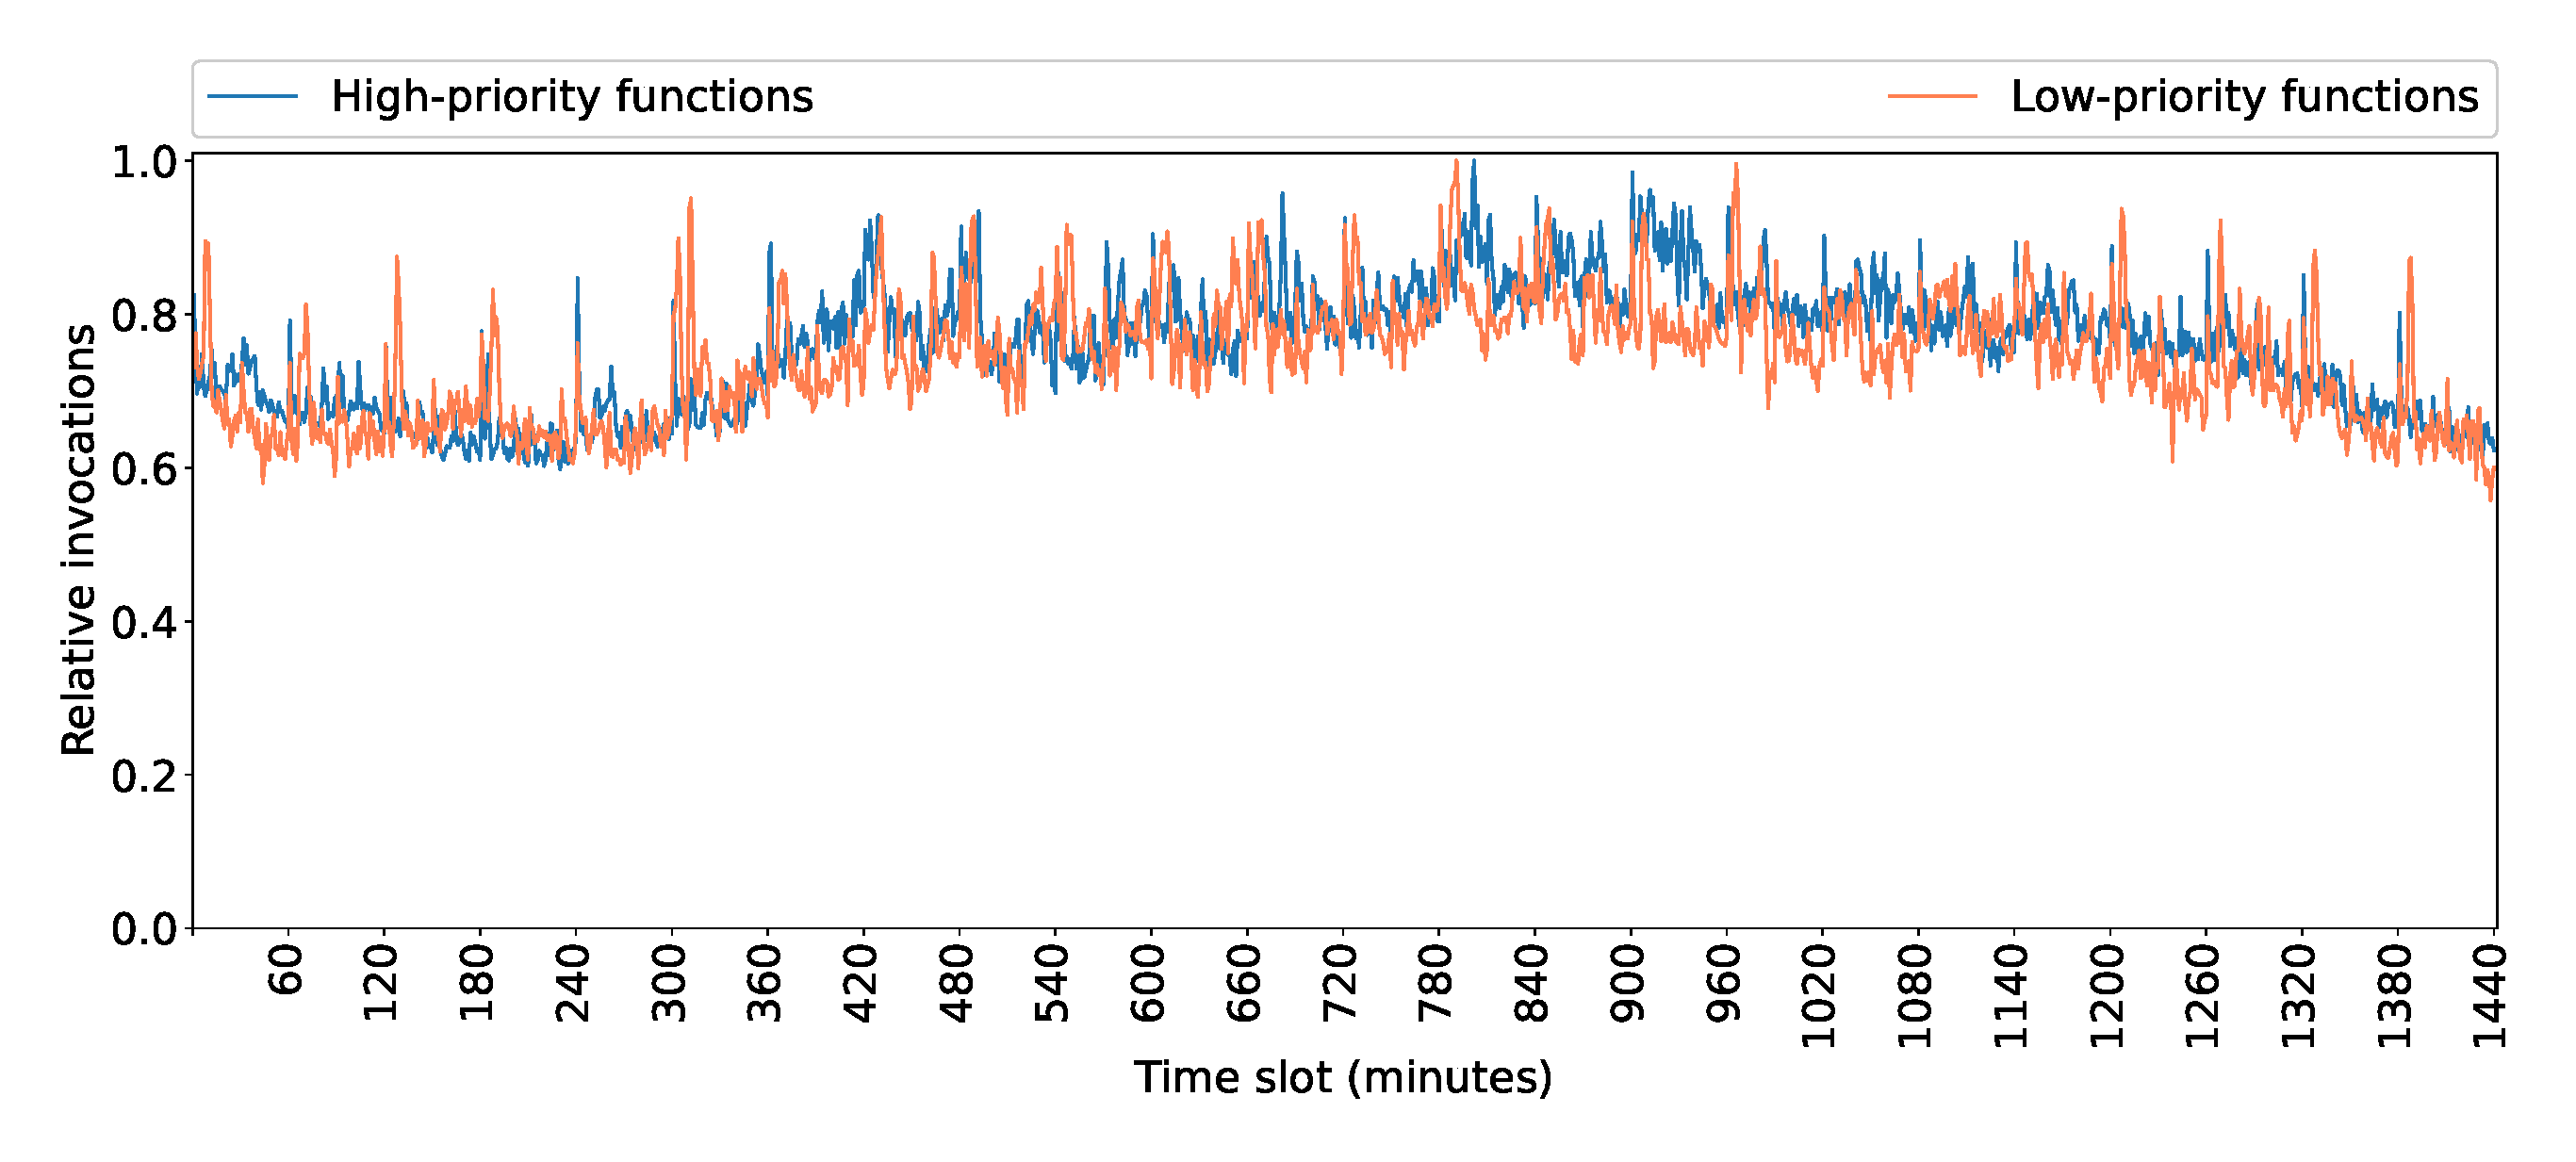
\includegraphics[width=\columnwidth]{../Figures/bursty-HighVsLowNormalized.eps}
    \caption{Invocations per minute, normalized to their peak, with functions divided into high- and low-priority groups.}
    \label{fig:bursty:highVsLowNormalized}
    % High-priority functions: 
    %   standard deviation :  0.0794
    %   IDC:  0.0083
    % Low-priority functions: 
    %   standard deviation :  0.0764
    %   IDC:  0.0079
\end{figure}
\end{comment}


%%% Local Variables:
%%% mode: latex
%%% TeX-master: "paper"
%%% End:
